%%%%%%%%%%%%%%%%%%%%%%%%%%%%%%%%%%%%%%%%%%%%%%%%%%%%%%%%%%%%%%%%%%%%%%%%%%%%%%%%%%
\begin{frame}[fragile]\frametitle{}
\begin{center}
{\Large Introduction to LangGraph}

{\tiny (Ref: LangGraph Crash Course - Harish Neel)}
\end{center}
\end{frame}

%%%%%%%%%%%%%%%%%%%%%%%%%%%%%%%%%%%%%%%%%%%%%%%%%%%%%%%%%%%%%%%%%%%%%%%%%%%%%%%%%%
\begin{frame}[fragile]\frametitle{}
\begin{center}
{\Large Background}
\end{center}
\end{frame}

%%%%%%%%%%%%%%%%%%%%%%%%%%%%%%%%%%%%%%%%%%%%%%%%%%%%%%%%%%%
\begin{frame}[fragile]\frametitle{The Evolution of LLM Applications}
      \begin{itemize}
        \item \textbf{Early Days}: Simple prompt-response patterns with single LLM calls
        \item \textbf{Challenge}: Real-world problems require multiple steps, decisions, and tool usage
        \item \textbf{Question}: How do we give LLMs more capability while maintaining control?
        \item \textbf{Journey}: From deterministic code → intelligent chains → autonomous agents
        \item \textbf{Core Tension}: Freedom vs Reliability
        \begin{itemize}
            \item More autonomy = More capable, but less predictable
            \item More structure = More reliable, but less flexible
        \end{itemize}
        \item \textbf{Goal}: Find the sweet spot between flexibility and control
      \end{itemize}
\end{frame}


%%%%%%%%%%%%%%%%%%%%%%%%%%%%%%%%%%%%%%%%%%%%%%%%%%%%%%%%%%%
\begin{frame}[fragile]\frametitle{Levels of Autonomy/Agency/Freedom: Overview}
      \begin{itemize}
        \item Think of autonomy as a spectrum from rigid to flexible
        \item Each level trades off control for capability
        \item Understanding these levels helps you choose the right tool
        \item \textbf{The Spectrum}:
        \begin{enumerate}
            \item Code: No autonomy, 100\% deterministic
            \item LLM Call: Single intelligent decision
            \item Chains: Sequential reasoning
            \item Routers: Conditional branching
			\item State: Workflow modeling with Cycles
            \item Agents: Autonomous decision-making with loops
        \end{enumerate}
        \item LangGraph enables 'State' level
      \end{itemize}
\end{frame}

%%%%%%%%%%%%%%%%%%%%%%%%%%%%%%%%%%%%%%%%%%%%%%%%%%%%%%%%%%%
\begin{frame}[fragile]\frametitle{Level 1-2: Code and Single LLM Calls}
      \begin{itemize}
        \item \textbf{Level 1: Pure Code}:
        \begin{itemize}
            \item Example: \lstinline|if temperature > 30: return "It's hot"| 
            \item No autonomy, 100\% deterministic, predictable
            \item Problem: Must anticipate every scenario
            \item Use case: Simple rule-based logic
        \end{itemize}
        \item \textbf{Level 2 - Single LLM Call}:
        \begin{itemize}
            \item Example: "Summarize this article" → LLM → Summary
            \item One input one output. One atomic task, limited reasoning
            \item Problem: Trying to do everything in one shot. Cannot break down complex tasks
            \item Use case: Text generation, classification, extraction
        \end{itemize}
        \item \textbf{Limitation}: Both lack multi-step reasoning capability
      \end{itemize}
\end{frame}

%%%%%%%%%%%%%%%%%%%%%%%%%%%%%%%%%%%%%%%%%%%%%%%%%%%%%%%%%%%
\begin{frame}[fragile]\frametitle{Level 3: Chains: Sequential Reasoning}
      \begin{itemize}
        \item \textbf{What}: Unidirectional sequence of LLM operations, so multiple experts one after another. Breaking down task is possible now.
        \item \textbf{Example: Customer Support}:
        \begin{itemize}
            \item Step 1: Classify intent (complaint/question/request)
            \item Step 2: Extract key information (order ID, issue)
            \item Step 3: Generate appropriate response
        \end{itemize}
        \item \textbf{Flow}: A → B → C → End (no branching, no loops)
        \item \textbf{Advantages}: Predictable, reliable, easy to debug
        \item \textbf{Limitations}: 
        \begin{itemize}
            \item Cannot adapt to different scenarios
            \item No conditional logic or branching
            \item Fixed execution path regardless of context
        \end{itemize}
        \item Like an assembly line, efficient but inflexible
      \end{itemize}
\end{frame}

%%%%%%%%%%%%%%%%%%%%%%%%%%%%%%%%%%%%%%%%%%%%%%%%%%%%%%%%%%%
\begin{frame}[fragile]\frametitle{Level 4: Routers: Conditional Branching}
      \begin{itemize}
        \item \textbf{What}: Chains with decision points, but still unidirectional
        \item \textbf{Example: Document Processing}:
        \begin{itemize}
            \item Analyze document type, LLM/ML, decision making (invoice/contract/email)
            \item IF invoice → Extract line items → Calculate total
            \item IF contract → Extract parties → Identify key terms
            \item IF email → Classify urgency → Route to handler
        \end{itemize}
        \item \textbf{Flow}: Decision node routes to specialized chains
        \item \textbf{Advantages}: Handles different scenarios, specialized processing
        \item \textbf{Limitations}:
        \begin{itemize}
            \item Still no loops or backward flow
            \item Cannot learn from mistake, cannot revisit back
            \item One-way path through the system
        \end{itemize}
        \item Like a train switching tracks - more flexible but still one direction
      \end{itemize}
\end{frame}

%%%%%%%%%%%%%%%%%%%%%%%%%%%%%%%%%%%%%%%%%%%%%%%%%%%%%%%%%%%
\begin{frame}[fragile]\frametitle{Level 5: State: Flow with Loops}
      \begin{itemize}
        \item \textbf{What}: State machines are Routers who can branch and loop.
        \item \textbf{Example: Content Creator}:
        \begin{itemize}
            \item Given a theme to write on
			\item HEAD can sending it for LinkedIn article writing, 
			\item Once done, we can have Human-approval, if not approved go back to the HEAD. Revise, iterate till approved.
			\item Once approved send to other forms such as Blog post, Twitter announcement post etc.
        \end{itemize}
        \item \textbf{Key Features}: 
        \begin{itemize}
            \item Can have human-in-loop for approval
			\item Multi-Agent systems
			\item Advanced Memory Management
			\item Can go back in history and explore better/alternate paths
        \end{itemize}		
        \item \textbf{Challenge}: Flow has to be prescribed, not full autonomy.
        \item \textbf{This is LangGraph}
      \end{itemize}
\end{frame}

%%%%%%%%%%%%%%%%%%%%%%%%%%%%%%%%%%%%%%%%%%%%%%%%%%%%%%%%%%%%%%%%%%%%%%%%%%%%%%%%%%
\begin{frame}[fragile]\frametitle{Level 5: State: Flow with Loops}
\begin{center}
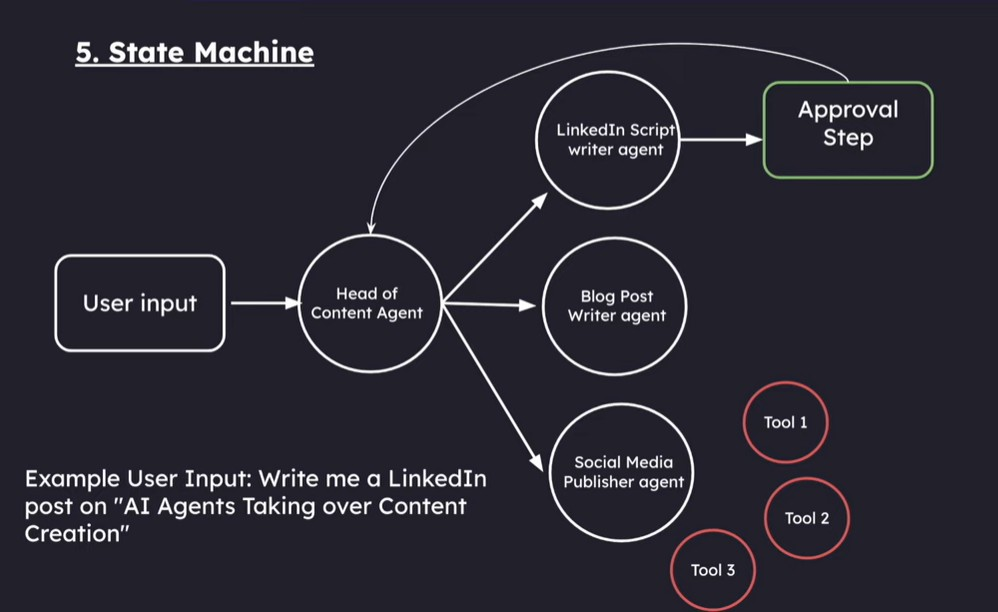
\includegraphics[width=0.9\linewidth,keepaspectratio]{langgraph24}

{\tiny (Ref: LangGraph Crash Course - Harish Neel)}
\end{center}	  
\end{frame}

%%%%%%%%%%%%%%%%%%%%%%%%%%%%%%%%%%%%%%%%%%%%%%%%%%%%%%%%%%%
\begin{frame}[fragile]\frametitle{Level 6: Agents: Autonomous with Loops}
      \begin{itemize}
        \item \textbf{What}: State machines with independent thinking, can loop and branch
        \item \textbf{Example - Research Assistant}:
        \begin{itemize}
            \item User: "Analyze SpaceX's latest launch success rate"
            \item Agent thinks: "I need current data and historical context"
            \item Action 1: Search web for latest SpaceX launches
            \item Observation: Found data but it's incomplete
            \item Action 2: Search for historical launch records
            \item Observation: Now have full picture
            \item Final answer: Synthesize findings into analysis
        \end{itemize}
        \item \textbf{Key Features}: Think → Act → Observe → Decide → Repeat
        \item \textbf{Challenge}: Can loop infinitely if not controlled
      \end{itemize}
\end{frame}

%%%%%%%%%%%%%%%%%%%%%%%%%%%%%%%%%%%%%%%%%%%%%%%%%%%%%%%%%%%%%%%%%%%%%%%%%%%%%%%%%%
\begin{frame}[fragile]\frametitle{Levels of Autonomy in LLM Applications}
\begin{center}
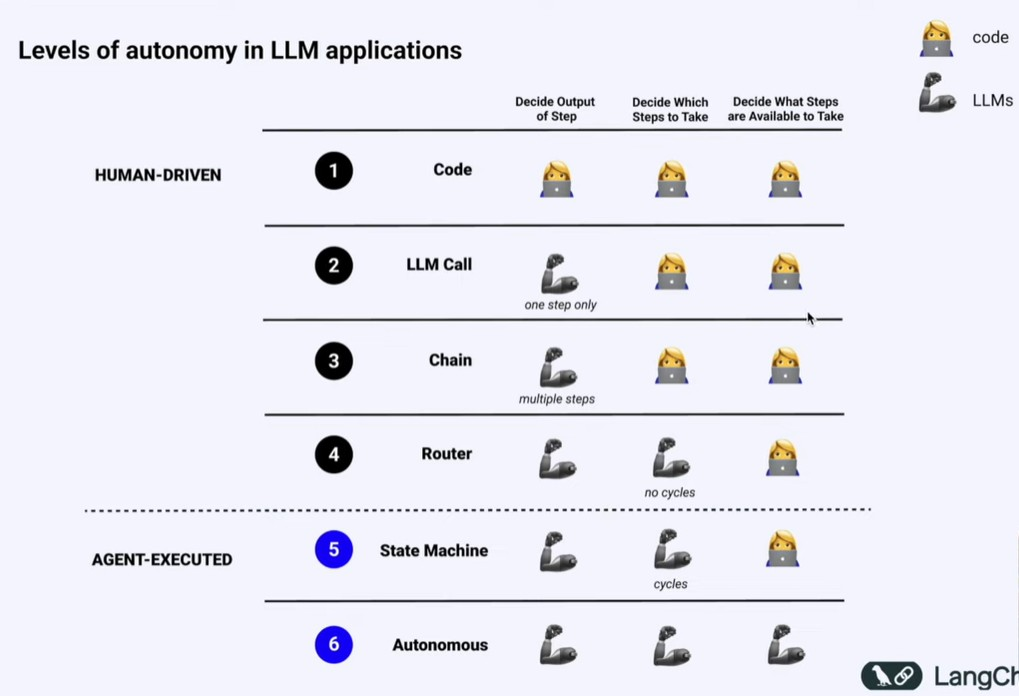
\includegraphics[width=0.8\linewidth,keepaspectratio]{langgraph5}

{\tiny (Ref: LangGraph Crash Course - Harish Neel)}
\end{center}	  

LLM (What AI decides) vs Code (What we prescribe/program)

\end{frame}

%%%%%%%%%%%%%%%%%%%%%%%%%%%%%%%%%%%%%%%%%%%%%%%%%%%%%%%%%%%
\begin{frame}[fragile]\frametitle{Human vs Agent Driven}
      \begin{itemize}
        \item 1-4 Human driven vs 5-6 Agent driven
		\item Why '5' ie 'State' agent driven? and not '3' or '4' where LLM is playing a part.
		\item A chain or a router is unidirectional hence it is not an agent
		\item A state machine can  go back in the flow as we have cycles and the flow is
controlled by the llm hence it is called an agent. 
		\item '3-4'has no self-correction, no training/learning, no refinement. That's intelligence. That's Agent.
      \end{itemize}
\end{frame}

%%%%%%%%%%%%%%%%%%%%%%%%%%%%%%%%%%%%%%%%%%%%%%%%%%%%%%%%%%%%%%%%%%%%%%%%%%%%%%%%%%
\begin{frame}[fragile]\frametitle{}
\begin{center}
{\Large Introduction to LangGraph}
\end{center}
\end{frame}

%%%%%%%%%%%%%%%%%%%%%%%%%%%%%%%%%%%%%%%%%%%%%%%%%%%%%%%%%%%
\begin{frame}[fragile]\frametitle{What is LangGraph?}

\begin{center}

\includegraphics[width=\linewidth,keepaspectratio]{langgraph14}
\end{center}


      \begin{itemize}
        \item LangGraph is an extension of the popular LangChain library. 
		\item Allows you to create AI applications that can perform multiple steps, make decisions, and maintain information across those steps. 
		\item Think of it like building a flowchart for your AI to follow.
      \end{itemize}
 

\end{frame}

%%%%%%%%%%%%%%%%%%%%%%%%%%%%%%%%%%%%%%%%%%%%%%%%%%%%%%%%%%%
\begin{frame}[fragile]\frametitle{Why LangGraph? - The Comprehensive Pitch}
      \begin{itemize}
        \item \textbf{Problem}: Traditional chains are too rigid, pure agents are too unpredictable
        \item \textbf{Solution}: LangGraph provides controlled flexibility through graph-based state machines
        \item \textbf{Key Benefits}:
        \begin{itemize}
            \item Explicit control flow with loops, branches, and conditional logic
            \item Built-in state persistence for long-running workflows
            \item Human-in-the-loop capabilities at any point
            \item Streaming support for real-time feedback
            \item Production-ready with debugging and observability
        \end{itemize}
        \item \textbf{Use Cases}: Multi-step reasoning, workflow automation, complex decision trees, collaborative agents
        \item \textbf{Result}: Reliable autonomous systems that combine flexibility with predictability
      \end{itemize}
\end{frame}

%%%%%%%%%%%%%%%%%%%%%%%%%%%%%%%%%%%%%%%%%%%%%%%%%%%%%%%%%%%
\begin{frame}[fragile]\frametitle{How is LangGraph Different?}


      \begin{itemize}
        \item Gives you more control over how your AI makes decisions
        \item Allows your AI to revisit previous steps if needed
        \item Makes it easier to add human oversight at specific points
        \item Integrates smoothly with other LangChain tools
      \end{itemize}


\begin{center}
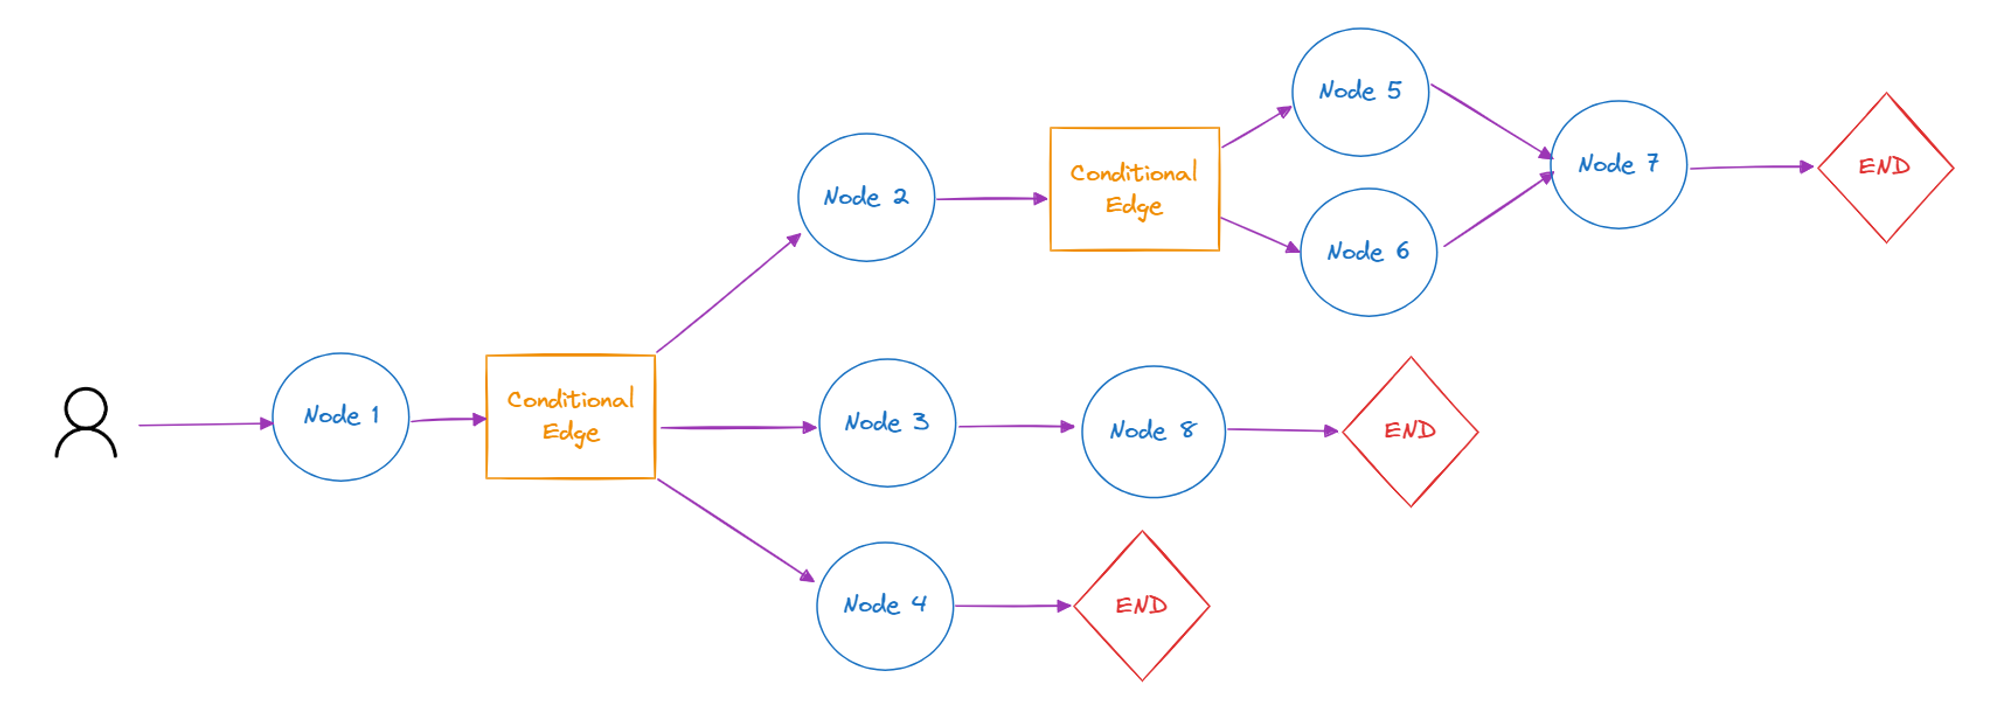
\includegraphics[width=\linewidth,keepaspectratio]{langgraph15}
\end{center}

\end{frame}

%%%%%%%%%%%%%%%%%%%%%%%%%%%%%%%%%%%%%%%%%%%%%%%%%%%%%%%%%%%
\begin{frame}[fragile]\frametitle{Agents in LangChain vs LangGraph}

\begin{columns}
    \begin{column}[T]{0.6\linewidth}
      \begin{itemize}
        \item \textbf{LangChain Agents (AgentExecutor)}:
        \begin{itemize}
            \item Black-box execution with limited control
            \item Fixed ReAct pattern implementation (TAO: Think-Action-Observe loop till we get the final answer)
            \item Cannot pause, resume, or modify mid-execution
            \item No state persistence across sessions
            \item Prone to infinite loops without guardrails
        \end{itemize}
        \item \textbf{LangGraph Agents}:
        \begin{itemize}
            \item White-box with full visibility into execution
            \item Custom patterns beyond ReAct
            \item Pause, resume, edit state at any node
            \item Persistent state with checkpointing
            \item Explicit cycle limits and control flow
        \end{itemize}
        \item \textbf{Bottom Line}: LangChain agents for simple tasks, LangGraph for production systems
      \end{itemize}

    \end{column}
    \begin{column}[T]{0.4\linewidth}
\begin{center}
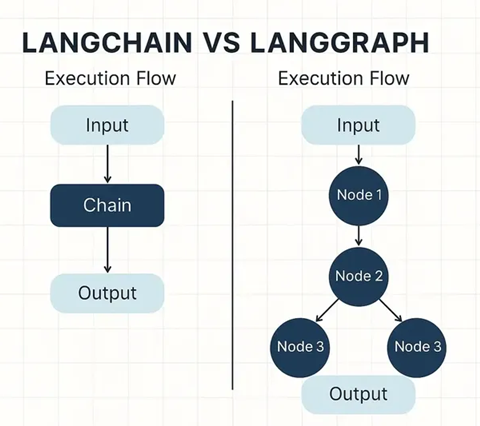
\includegraphics[width=\linewidth,keepaspectratio]{langgraph16}
\end{center}
    \end{column}
  \end{columns}
  
  

\end{frame}

%%%%%%%%%%%%%%%%%%%%%%%%%%%%%%%%%%%%%%%%%%%%%%%%%%%%%%%%%%%
\begin{frame}[fragile]\frametitle{Why Graph Structure Over Chains?}


      \begin{itemize}
        \item \textbf{Chains Limitation}: Linear, unidirectional flow - A → B → C → End
        \item \textbf{Real-World Problems}: Require branching, loops, and conditional paths
        \item \textbf{Graph Advantages}:
        \begin{itemize}
            \item Conditional branching: "If quality < threshold, loop back"
            \item Multiple paths: "Route to specialized nodes based on task type"
            \item Cycles: "Iterate until convergence or max iterations"
            \item Parallel execution: "Process multiple sub-tasks simultaneously"
        \end{itemize}
        \item \textbf{Research-Backed}: Most complex AI problem-solving papers use graph structures
        \item \textbf{Natural Fit}: Mirrors human problem-solving with think-act-observe-decide cycles
        \item Graphs provide flexibility while maintaining explicit control flow
      \end{itemize}

\end{frame}

%%%%%%%%%%%%%%%%%%%%%%%%%%%%%%%%%%%%%%%%%%%%%%%%%%%%%%%%%%%
\begin{frame}[fragile]\frametitle{Agentic Patterns: Autonomous vs Workflow Automation}
      \begin{itemize}
        \item \textbf{Autonomous Agents}:
        \begin{itemize}
            \item High-level goals with minimal constraints
            \item Self-directed exploration and decision-making
            \item Example: "Research this topic and write a report"
            \item Higher risk of unpredictability
        \end{itemize}
        \item \textbf{Workflow Automation Agents}:
        \begin{itemize}
            \item Structured processes with defined checkpoints
            \item Predictable paths with conditional logic
            \item Example: "Review email → Classify → Route → Draft response"
            \item Balance between automation and control
        \end{itemize}
        \item \textbf{LangGraph Sweet Spot}: Workflow automation with controlled autonomy
        \item Graphs enable explicit workflow definition while allowing intelligent decisions at each node
      \end{itemize}
\end{frame}

%%%%%%%%%%%%%%%%%%%%%%%%%%%%%%%%%%%%%%%%%%%%%%%%%%%%%%%%%%%%%%%%%%%%%%%%%%%%%%%%%%
\begin{frame}[fragile]\frametitle{}
\begin{center}
{\Large LangGraph Core Concepts}
\end{center}
\end{frame}

%%%%%%%%%%%%%%%%%%%%%%%%%%%%%%%%%%%%%%%%%%%%%%%%%%%%%%%%%%%%%%%%%%%%%%%%%%%%%%%%%%
\begin{frame}\frametitle{LangGraph Concepts}
\begin{itemize}
\item Model: Large Language Model that supports Function Calling
\item Tools: Actions taken by app - API calls, database operations, etc.
\item State: Information carried throughout the workflow (e.g., Message State)
\item Node: Executable logic container - a LangChain runnable or Tool invoker
\item Edge: Control flow of information - conditional or normal
\item Workflow: The graph with nodes and edges that can be invoked or streamed
\end{itemize}

\begin{center}
\includegraphics[width=0.8\linewidth,keepaspectratio]{langgraph2}
\end{center}	  
{\tiny (Ref: Introduction to LangGraph | Building an AI Generated Podcast - Prompt Circle AI)}
\end{frame}


%%%%%%%%%%%%%%%%%%%%%%%%%%%%%%%%%%%%%%%%%%%%%%%%%%%%%%%%%%%
\begin{frame}[fragile]\frametitle{LangGraph Fundamentals: Nodes, Edges \& State}


      \begin{itemize}
        \item \textbf{Nodes (N):} Individual processing steps as Python functions that transform state
        \item Each node encapsulates one sub-task: LLM calls, calculations, tool invocations
        \item \textbf{Edges (E):} Directed connections determining execution flow between nodes
        \item Edges can be linear or conditional routes based on current state
        \item \textbf{State (S):} Shared data object persisting throughout execution
        % \item State enables context and memory across workflow
        % \item StateGraph ties everything together with designated START and END nodes
        % \item Handles interactive, conditional loops that static chains struggle with
      \end{itemize}


\begin{center}
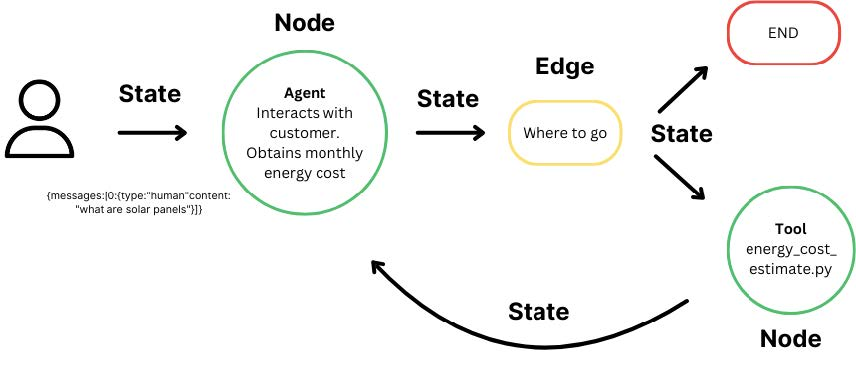
\includegraphics[width=0.6\linewidth,keepaspectratio]{langgraph19}

{\tiny (Ref: The Complete Guide to Building LangChain Agents)}
\end{center}

  

\end{frame}


%%%%%%%%%%%%%%%%%%%%%%%%%%%%%%%%%%%%%%%%%%%%%%%%%%%%%%%%%%%
\begin{frame}[fragile]\frametitle{Core Components: Nodes}

	  

      \begin{itemize}
        \item Fundamental execution units in the graph
        \item Each node represents a specific operation or LLM call
        \item Nodes contain the actual logic and processing
        \item Can be simple operations or complex LLM interactions
        \item Examples: Start Node, Generate Content, Evaluate Quality, Tool Invocation, End Node
      \end{itemize}


\begin{center}
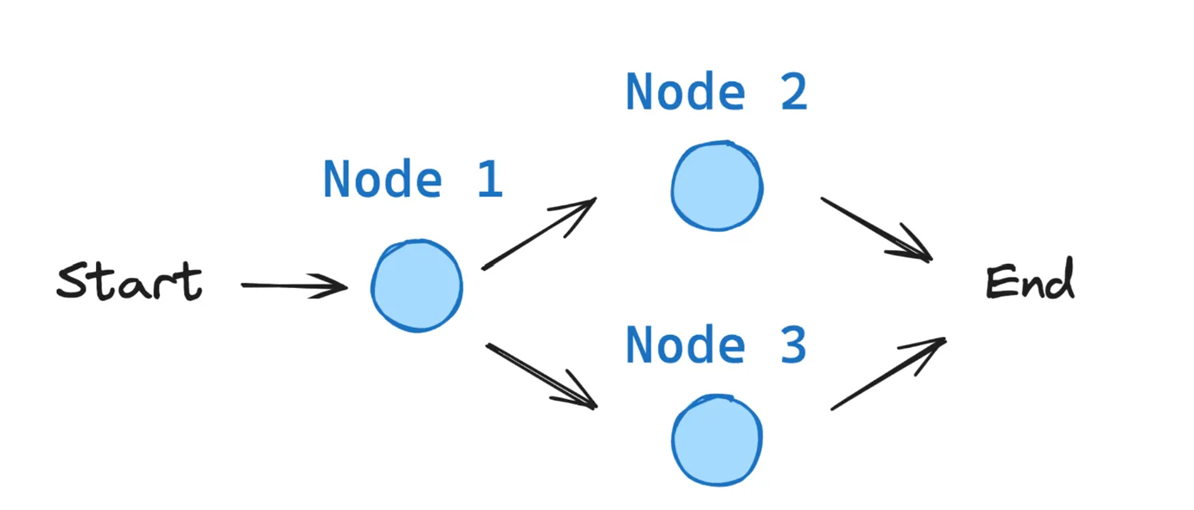
\includegraphics[width=0.8\linewidth,keepaspectratio]{langgraph20}

{\tiny (Ref: Building Simple LangGraph - Uss Varma)}
\end{center}
  
\end{frame}

%%%%%%%%%%%%%%%%%%%%%%%%%%%%%%%%%%%%%%%%%%%%%%%%%%%%%%%%%%%
\begin{frame}[fragile]\frametitle{Is Each Node an Agent or Is the Graph an Agent?}
      \begin{itemize}
        \item \textbf{The Graph is the Agent} - not individual nodes
        \item \textbf{Nodes are}: Individual processing units/functions
        \begin{itemize}
            \item Can be simple Python functions
            \item Can be LLM calls
            \item Can be tool invocations
            \item Can be sub-agents themselves
        \end{itemize}
        \item \textbf{The Graph as Agent}:
        \begin{itemize}
            \item The complete workflow represents the agent's behavior
            \item State flows through nodes, creating agent "memory"
            \item Control flow (edges) represents agent's decision-making
            \item Overall graph exhibits autonomous, goal-directed behavior
        \end{itemize}
        \item \textbf{Analogy}: Nodes are like neurons, the graph is the brain
        \item Individual nodes are stateless functions; the graph maintains state
      \end{itemize}
\end{frame}

%%%%%%%%%%%%%%%%%%%%%%%%%%%%%%%%%%%%%%%%%%%%%%%%%%%%%%%%%%%
\begin{frame}[fragile]\frametitle{What Can Nodes Do? - Part 1}
      \begin{itemize}
        \item \textbf{Nodes are Extremely Flexible} - any Python function
        \item \textbf{1. Simple LLM Calls}:
        \begin{itemize}
            \item Generate text, classify, extract information
            \item Example: `llm.invoke("Summarize this text")`
        \end{itemize}
        \item \textbf{2. RAG Operations}:
        \begin{itemize}
            \item Retrieve documents from vector database
            \item Rerank results
            \item Generate answers with retrieved context
            \item Example: Vector search → Context → LLM generation
        \end{itemize}
        \item \textbf{3. API Calls}:
        \begin{itemize}
            \item External service calls (weather, database, CRM)
            \item Example: Fetch customer data from Salesforce API
        \end{itemize}
      \end{itemize}
\end{frame}

%%%%%%%%%%%%%%%%%%%%%%%%%%%%%%%%%%%%%%%%%%%%%%%%%%%%%%%%%%%
\begin{frame}[fragile]\frametitle{What Can Nodes Do? - Part 2}
      \begin{itemize}
        \item \textbf{4. Tool-Calling Agents}:
        \begin{itemize}
            \item Node can itself be an agent with tools
            \item Example: Research node that uses search, calculator, Wikipedia tools
            \item Inner agent makes tool decisions, outer graph manages workflow
        \end{itemize}
        \item \textbf{5. Multi-Agent Nodes}:
        \begin{itemize}
            \item Node can coordinate multiple sub-agents
            \item Example: "Code Review" node with architect, tester, security agents
        \end{itemize}
        \item \textbf{6. Any Computation}:
        \begin{itemize}
            \item Data processing, calculations, file operations
            \item Validation, formatting, business logic
        \end{itemize}
        \item \textbf{Key Point}: Nodes are building blocks - combine them creatively
      \end{itemize}
\end{frame}


%%%%%%%%%%%%%%%%%%%%%%%%%%%%%%%%%%%%%%%%%%%%%%%%%%%%%%%%%%%
\begin{frame}[fragile]\frametitle{Core Components: Edges}


      \begin{itemize}
        \item Connections between nodes in the graph
        \item Represent the flow of execution from one node to another
        \item Define possible paths through the workflow
        \item Can be simple directional connections
        \item Ensure proper sequence of operations
      \end{itemize}


\begin{center}
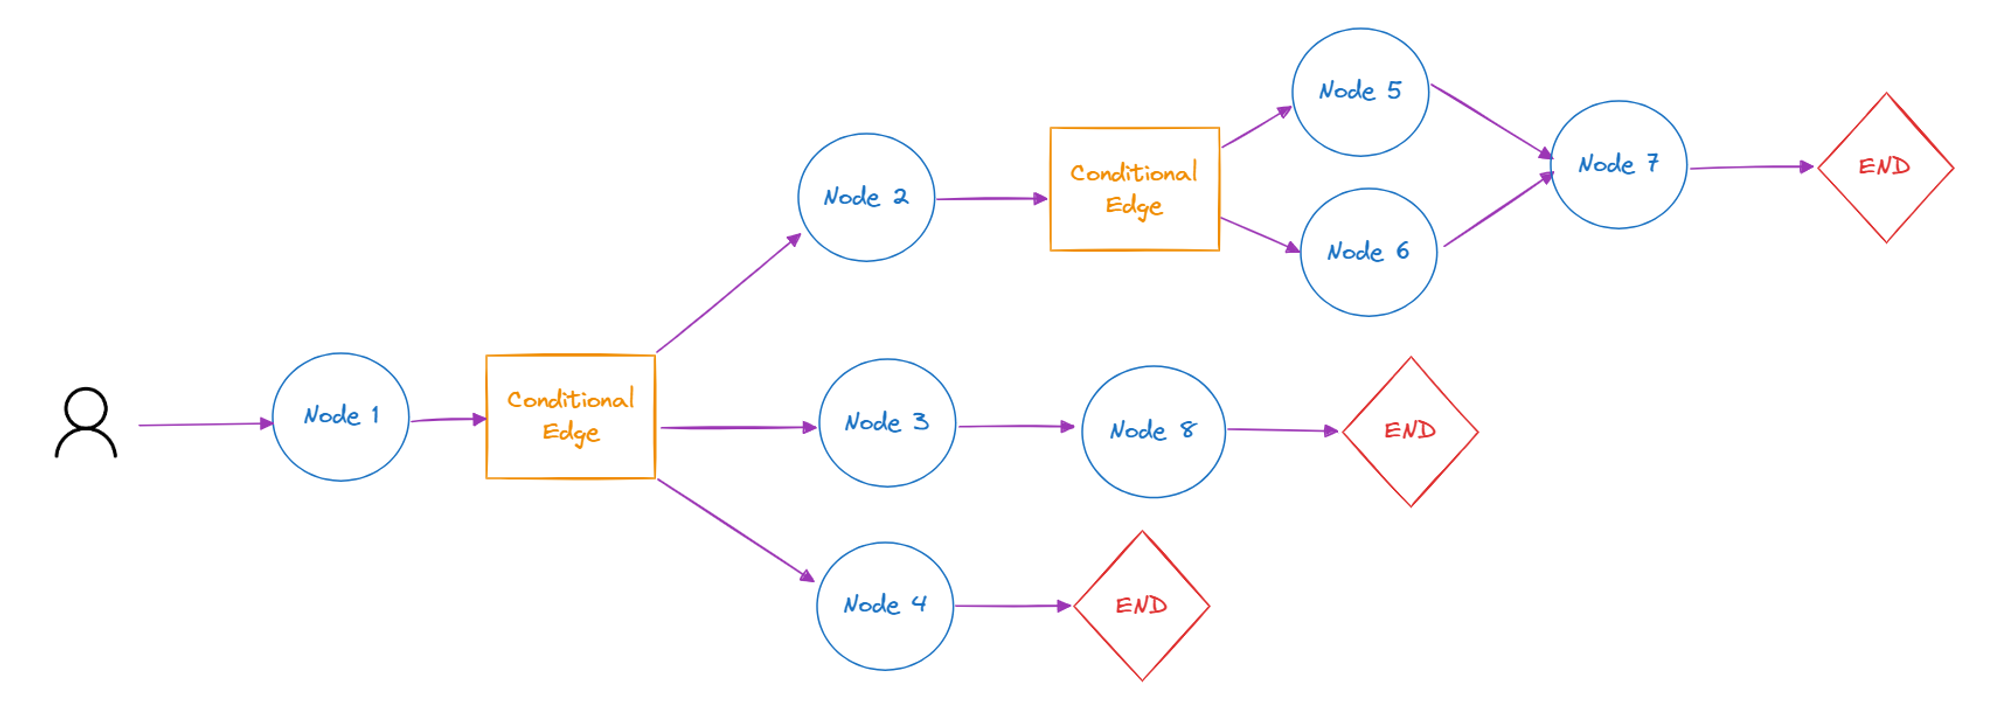
\includegraphics[width=\linewidth,keepaspectratio]{langgraph21}

{\tiny (Ref: A Comprehensive Guide About Langgraph: Code Included - Shivam Danawale)}
\end{center}
 
  

\end{frame}

%%%%%%%%%%%%%%%%%%%%%%%%%%%%%%%%%%%%%%%%%%%%%%%%%%%%%%%%%%%
\begin{frame}[fragile]\frametitle{Core Components: Conditional Edges}
      \begin{itemize}
        \item Decision points in the workflow
        \item Enable branching based on specific conditions
        \item Example: After generation, route to criticism OR end based on quality
        \item Represented by dotted lines in diagrams
        \item Allow for dynamic execution paths
        \item Essential for implementing loops and conditional branching
      \end{itemize}
\end{frame}

%%%%%%%%%%%%%%%%%%%%%%%%%%%%%%%%%%%%%%%%%%%%%%%%%%%%%%%%%%%
\begin{frame}[fragile]\frametitle{Core Components: State}
      \begin{itemize}
	    \item A central object updated over time by the nodes in the graph
        \item Maintains context throughout workflow execution
        \item Preserves information between node executions
        \item State contains: messages, intermediate results, iteration count, tool outputs
        \item Enables nodes to access and modify shared information
        \item Critical for maintaining workflow coherence
        \item Supports complex, stateful operations
      \end{itemize}
\end{frame}


%%%%%%%%%%%%%%%%%%%%%%%%%%%%%%%%%%%%%%%%%%%%%%%%%%%%%%%%%%%
\begin{frame}[fragile]\frametitle{LangGraph Key Features}
      \begin{itemize}
        \item \textbf{Looping and Branching}: Conditional statements and loop structures
        \item \textbf{State Persistence}: Automatic save/restore, pause and resume
        \item \textbf{Human-in-the-Loop}: Insert human review, state editing capabilities
        \item \textbf{Streaming Processing}: Real-time feedback on execution status
        \item \textbf{LangChain Integration}: Reuses existing components, LCEL support
        \item Provides controlled flexibility unlike pure React agents
        \item Production-ready with debugging and observability
      \end{itemize}
\end{frame}

%%%%%%%%%%%%%%%%%%%%%%%%%%%%%%%%%%%%%%%%%%%%%%%%%%%%%%%%%%%%%%%%%%%%%%%%%%%%%%%%%%
\begin{frame}[fragile]\frametitle{}
\begin{center}
{\Large Simple Example}
\end{center}
\end{frame}

%%%%%%%%%%%%%%%%%%%%%%%%%%%%%%%%%%%%%%%%%%%%%%%%%%%%%%%%%%%
\begin{frame}[fragile]\frametitle{Weather Checking Assistant}


      \begin{itemize}
        \item Greet the user
        \item Ask for their location
        \item Check the weather (simulated for this example)
        \item Provide a weather report
      \end{itemize}


\begin{center}
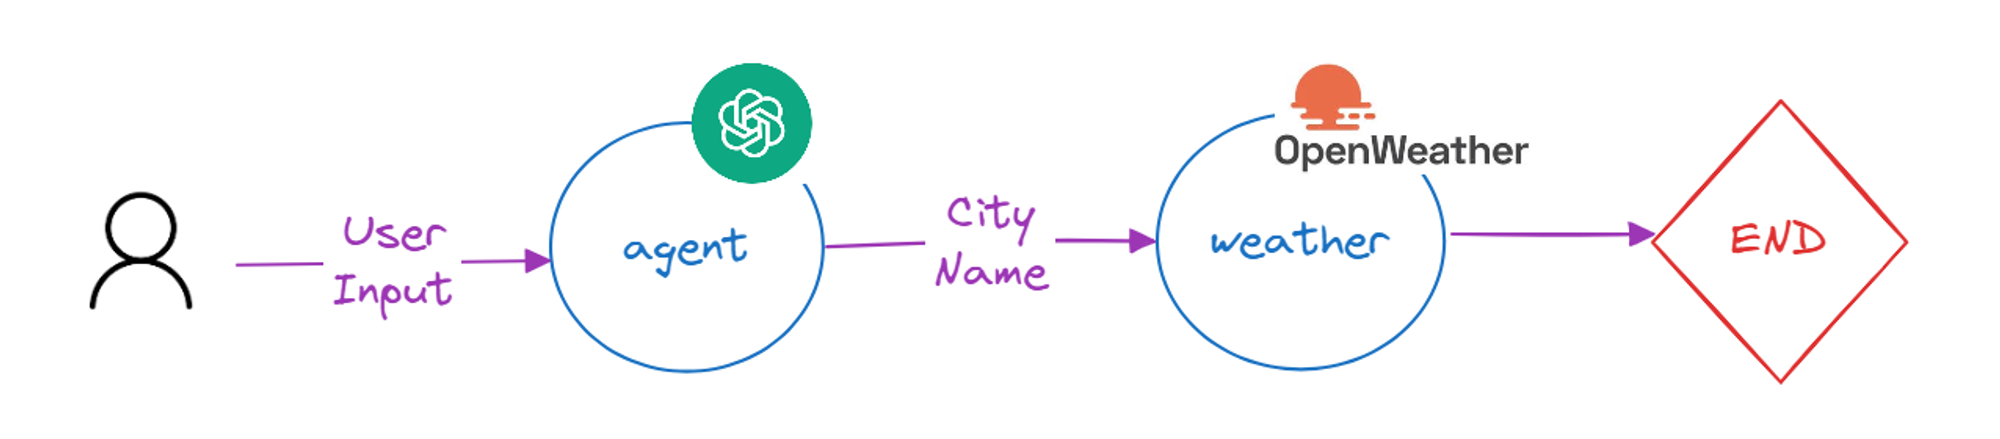
\includegraphics[width=\linewidth,keepaspectratio]{langgraph18}
\end{center}

  
  

\end{frame}

%%%%%%%%%%%%%%%%%%%%%%%%%%%%%%%%%%%%%%%%%%%%%%%%%%%%%%%%%%%
\begin{frame}[fragile]\frametitle{Code Part 1}
      \begin{lstlisting}[language=Python, basicstyle=\tiny]
import operator
from typing import TypedDict
from typing_extensions import Annotated
from langgraph.graph import StateGraph, END

# Define our state
class State(TypedDict):
    messages: Annotated[list, operator.add]
    location: str
    weather: str

# Create our graph
workflow = StateGraph(State)

# Define our nodes
def greet(state):
    return {"messages": [("ai", "Hello! I'm your weather assistant. Where are you located?")]}

def get_location(state):
    return {"location": state["messages"][-1][1]}

def check_weather(state):
    # In a real app, we'd call a weather API here
    weather = "sunny" if "new york" in state["location"].lower() else "rainy"
    return {"weather": weather}

def report_weather(state):
    return {"messages": [
        ("ai", f"The weather in {state['location']} is {state['weather']}. Can I help you with anything else?")]}
      \end{lstlisting}
\end{frame}


%%%%%%%%%%%%%%%%%%%%%%%%%%%%%%%%%%%%%%%%%%%%%%%%%%%%%%%%%%%
\begin{frame}[fragile]\frametitle{Code Part 2}
      \begin{lstlisting}[language=Python, basicstyle=\tiny]
# Add nodes to our graph
workflow.add_node("greet", greet)
workflow.add_node("get_location", get_location)
workflow.add_node("check_weather", check_weather)
workflow.add_node("report_weather", report_weather)

# Connect our nodes
workflow.set_entry_point("greet")
workflow.add_edge("greet", "get_location")
workflow.add_edge("get_location", "check_weather")
workflow.add_edge("check_weather", "report_weather")
workflow.add_edge("report_weather", END)

# Compile our graph
app = workflow.compile()

# Run our app
inputs = {"messages": [("human", "Hi, I'd like to check the weather.")]}
for output in app.stream(inputs):
    for key, value in output.items():
        print(f"{key}: {value}")
	
# Printing the graph in ASCII	
ascii_graph = app.get_graph().draw_ascii()
print(ascii_graph)	
	
      \end{lstlisting}
\end{frame}


%%%%%%%%%%%%%%%%%%%%%%%%%%%%%%%%%%%%%%%%%%%%%%%%%%%%%%%%%%%%%%%%%%%%%%%%%%%%%%%%%%
\begin{frame}[fragile]\frametitle{}
\begin{center}
{\Large Getting Started}
\end{center}
\end{frame}

%%%%%%%%%%%%%%%%%%%%%%%%%%%%%%%%%%%%%%%%%%%%%%%%%%%%%%%%%%%
\begin{frame}[fragile]\frametitle{Installation}
LangGraph requires Python 3.8 or later. 

      \begin{lstlisting}
pip install -U langgraph

python -c "import langgraph; print(langgraph.__version__)"
      \end{lstlisting}
\end{frame}

%%%%%%%%%%%%%%%%%%%%%%%%%%%%%%%%%%%%%%%%%%%%%%%%%%%%%%%%%%%
\begin{frame}[fragile]\frametitle{Step 1: Define State}


      \begin{lstlisting}
from typing import Annotated
from typing_extensions import TypedDict
from langgraph.graph import StateGraph
from langgraph.graph.message import add_messages
class State(TypedDict):
    # messages have the type "list".
    # The add_messages function appends messages to the list, rather than overwriting them
    messages: Annotated[list, add_messages]
graph_builder = StateGraph(State)
      \end{lstlisting}
\end{frame}


%%%%%%%%%%%%%%%%%%%%%%%%%%%%%%%%%%%%%%%%%%%%%%%%%%%%%%%%%%%
\begin{frame}[fragile]\frametitle{Step 2: Initialize an LLM and add it as a Chatbot node}


      \begin{lstlisting}
from langchain_openai import AzureChatOpenAI
llm = AzureChatOpenAI(
    openai_api_version=os.environ["AZURE_OPENAI_API_VERSION"],
    azure_deployment=os.environ["AZURE_OPENAI_CHAT_DEPLOYMENT_NAME"],
)
def chatbot(state: State):
    return {"messages": [llm.invoke(state["messages"])]}
	
graph_builder.add_node("chatbot", chatbot)
      \end{lstlisting}
\end{frame}

%%%%%%%%%%%%%%%%%%%%%%%%%%%%%%%%%%%%%%%%%%%%%%%%%%%%%%%%%%%
\begin{frame}[fragile]\frametitle{Step 3: Set edges}

      \begin{lstlisting}
# Set entry and finish points
graph_builder.set_entry_point("chatbot")
graph_builder.set_finish_point("chatbot")
      \end{lstlisting}
\end{frame}

%%%%%%%%%%%%%%%%%%%%%%%%%%%%%%%%%%%%%%%%%%%%%%%%%%%%%%%%%%%
\begin{frame}[fragile]\frametitle{Step 4: Compile and Visualize the Graph}

\lstinline|pip install graphviz|

\begin{columns}
    \begin{column}[T]{0.8\linewidth}
      \begin{lstlisting}[language=Python, basicstyle=\small]
import os

png_graph = graph.get_graph().draw_mermaid_png()
with open("my_graph.png", "wb") as f:
    f.write(png_graph)

print(f"Graph saved as 'my_graph.png' in {os.getcwd()}")
      \end{lstlisting}

    \end{column}
    \begin{column}[T]{0.2\linewidth}
\begin{center}
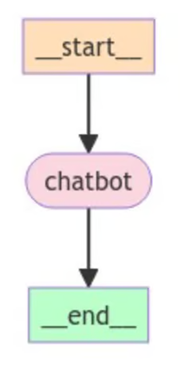
\includegraphics[width=\linewidth,keepaspectratio]{langgraph13.png}
\end{center}
    \end{column}
  \end{columns}
  
\end{frame}

%%%%%%%%%%%%%%%%%%%%%%%%%%%%%%%%%%%%%%%%%%%%%%%%%%%%%%%%%%%
\begin{frame}[fragile]\frametitle{Step 5: Run the chatbot}

 Implement a loop to continuously prompt the user for input, process it through the graph, and print the assistant's response. The loop exits when the user types "quit", "exit", or "q".
 
      \begin{lstlisting}
# Run the chatbot
while True:
    user_input = input("User: ")
    if user_input.lower() in ["quit", "exit", "q"]:
        print("Goodbye!")
        break
    for event in graph.stream({"messages": [("user", user_input)]}):
        for value in event.values():
            print("Assistant:", value["messages"][-1].content)
      \end{lstlisting}
\end{frame}

%%%%%%%%%%%%%%%%%%%%%%%%%%%%%%%%%%%%%%%%%%%%%%%%%%%%%%%%%%%%%%%%%%%%%%%%%%%%%%%%%%
\begin{frame}[fragile]\frametitle{}
\begin{center}
{\Large Tutorial: Workflow Automation}
\end{center}
\end{frame}

%%%%%%%%%%%%%%%%%%%%%%%%%%%%%%%%%%%%%%%%%%%%%%%%%%%%%%%%%%%
\begin{frame}[fragile]\frametitle{Tutorial: Email Classification Workflow}
      \begin{itemize}
        \item \textbf{Goal}: Automate email triage with classification and routing
        \item \textbf{Workflow Steps}:
        \begin{enumerate}
            \item Read incoming email
            \item Classify as spam/legitimate using LLM
            \item Route to spam handler or response drafter
            \item Draft response for legitimate emails
            \item Send notification
        \end{enumerate}
        \item Demonstrates conditional routing and structured workflow
        \item Shows how graphs handle if/else logic naturally
      \end{itemize}
\end{frame}

%%%%%%%%%%%%%%%%%%%%%%%%%%%%%%%%%%%%%%%%%%%%%%%%%%%%%%%%%%%
\begin{frame}[fragile]\frametitle{Step 1: Define State}

      \begin{itemize}
        \item State holds all information passed between nodes
        \item Type hints ensure clarity and validation
      \end{itemize}
	  
	  
      \begin{lstlisting}[language=Python, basicstyle=\small]
from typing import List, Dict
from pydantic import BaseModel

class EmailState(BaseModel):
    email_content: str = ""
    is_spam: bool = False
    category: str = ""
    draft_response: str = ""
    messages: List[Dict[str, str]] = []
      \end{lstlisting}
      

\end{frame}

%%%%%%%%%%%%%%%%%%%%%%%%%%%%%%%%%%%%%%%%%%%%%%%%%%%%%%%%%%%
\begin{frame}[fragile]\frametitle{Step 2: Create Node Functions}
      \begin{lstlisting}[language=Python, basicstyle=\tiny]
from langchain_openai import ChatOpenAI

llm = ChatOpenAI(model="gpt-4", temperature=0)

def read_email(state: EmailState) -> EmailState:
    # In production, read from email API
    return state

def classify_email(state: EmailState) -> EmailState:
    prompt = f"Classify this email as spam or legitimate:\n{state.email_content}\nRespond with only 'spam' or 'legitimate'."
    response = llm.invoke(prompt)
    is_spam = "spam" in response.content.lower()
    return EmailState(
        email_content=state.email_content,
        is_spam=is_spam,
        messages=state.messages + [{"role": "classifier", "content": response.content}]
    )

def handle_spam(state: EmailState) -> EmailState:
    return EmailState(**state.dict(), 
        messages=state.messages + [{"role": "system", "content": "Email marked as spam"}])

def draft_response(state: EmailState) -> EmailState:
    prompt = f"Draft a professional response to:\n{state.email_content}"
    response = llm.invoke(prompt)
    return EmailState(**state.dict(), 
        draft_response=response.content,
        messages=state.messages + [{"role": "drafter", "content": response.content}])
      \end{lstlisting}
\end{frame}

%%%%%%%%%%%%%%%%%%%%%%%%%%%%%%%%%%%%%%%%%%%%%%%%%%%%%%%%%%%
\begin{frame}[fragile]\frametitle{Step 3: Define Routing Logic}

      \begin{itemize}
        \item Routing function decides next node based on state
        \item Returns the name of the target node
        \item Enables dynamic workflow execution
      \end{itemize}
	  
      \begin{lstlisting}[language=Python, basicstyle=\tiny]
def route_email(state: EmailState) -> str:
    """Conditional routing based on classification"""
    if state.is_spam:
        return "spam_handler"
    else:
        return "response_drafter"
      \end{lstlisting}
      

\end{frame}

%%%%%%%%%%%%%%%%%%%%%%%%%%%%%%%%%%%%%%%%%%%%%%%%%%%%%%%%%%%
\begin{frame}[fragile]\frametitle{Step 4: Build the Graph}
      \begin{lstlisting}[language=Python, basicstyle=\tiny]
from langgraph.graph import StateGraph, END

# Create graph
workflow = StateGraph(EmailState)

# Add nodes
workflow.add_node("read_email", read_email)
workflow.add_node("classify_email", classify_email)
workflow.add_node("spam_handler", handle_spam)
workflow.add_node("response_drafter", draft_response)

# Add edges
workflow.set_entry_point("read_email")
workflow.add_edge("read_email", "classify_email")
workflow.add_conditional_edges(
    "classify_email",
    route_email,
    {"spam_handler": "spam_handler", 
     "response_drafter": "response_drafter"}
)
workflow.add_edge("spam_handler", END)
workflow.add_edge("response_drafter", END)

# Compile
app = workflow.compile()
      \end{lstlisting}
\end{frame}

%%%%%%%%%%%%%%%%%%%%%%%%%%%%%%%%%%%%%%%%%%%%%%%%%%%%%%%%%%%
\begin{frame}[fragile]\frametitle{Step 5: Run the Workflow}

      \begin{itemize}
        \item Workflow executes automatically with proper routing
        \item State carries results through entire execution
      \end{itemize}
	  
      \begin{lstlisting}[language=Python, basicstyle=\small]
# Test with legitimate email
state = EmailState(
    email_content="Hello, I'd like to schedule a meeting to discuss the project timeline."
)
result = app.invoke(state)
print(f"Is Spam: {result.is_spam}")
print(f"Draft Response: {result.draft_response}")

# Test with spam email
spam_state = EmailState(
    email_content="URGENT! You've won $1M! Click here now!!!"
)
spam_result = app.invoke(spam_state)
print(f"Is Spam: {spam_result.is_spam}")
      \end{lstlisting}
      

\end{frame}

%%%%%%%%%%%%%%%%%%%%%%%%%%%%%%%%%%%%%%%%%%%%%%%%%%%%%%%%%%%
\begin{frame}[fragile]\frametitle{Tutorial Takeaways}
      \begin{itemize}
        \item \textbf{Clear Structure}: Graph makes workflow explicit and understandable
        \item \textbf{Conditional Logic}: Natural if/else through routing functions
        \item \textbf{State Management}: Single state object tracks entire process
        \item \textbf{Extensibility}: Easy to add new nodes (e.g., "urgent" category)
        \item \textbf{Debugging}: Can inspect state at each node
        \item \textbf{Production-Ready}: Add checkpointing, error handling, retries
        \item This pattern scales to complex multi-step workflows
      \end{itemize}
\end{frame}

%%%%%%%%%%%%%%%%%%%%%%%%%%%%%%%%%%%%%%%%%%%%%%%%%%%%%%%%%%%%%%%%%%%%%%%%%%%%%%%%%%
\begin{frame}[fragile]\frametitle{}
\begin{center}
{\Large Real-World Applications}
\end{center}
\end{frame}

%%%%%%%%%%%%%%%%%%%%%%%%%%%%%%%%%%%%%%%%%%%%%%%%%%%%%%%%%%%%%%%%%%%%%%%%%%%%%%%%%%
\begin{frame}\frametitle{Example: Podcast Generator}
\begin{center}
\includegraphics[width=0.8\linewidth,keepaspectratio]{langgraph3}
\end{center}	  
{\tiny (Ref: Introduction to LangGraph | Building an AI Generated Podcast - Prompt Circle AI)}

Code at https://github.com/hollaugo/langgraph-framework-tutorial
\end{frame}

%%%%%%%%%%%%%%%%%%%%%%%%%%%%%%%%%%%%%%%%%%%%%%%%%%%%%%%%%%%%%%%%%%%%%%%%%%%%%%%%%%
\begin{frame}[fragile]\frametitle{Example: News Aggregator}
\begin{center}
\includegraphics[width=0.8\linewidth,keepaspectratio]{langgraph4}
\end{center}	

Code: https://github.com/rajib76/multi\_agent/01\_how\_to\_langgraph\_example\_01.py

{\tiny (Ref: Langgraph: The Agent Orchestrator - Rajib Deb)}
\end{frame}

%%%%%%%%%%%%%%%%%%%%%%%%%%%%%%%%%%%%%%%%%%%%%%%%%%%%%%%%%%%
\begin{frame}[fragile]\frametitle{Best Practices}
      \begin{itemize}
        \item \textbf{State Design}: Keep simple and clear, use type hints, only necessary information
        \item \textbf{Node Functions}: Single responsibility, handle exceptions, return new state objects
        \item \textbf{Edge Design}: Clear conditional logic, avoid complex cycles, consider all paths
        \item \textbf{Error Handling}: Add at critical nodes, provide fallback mechanisms, log errors
        \item \textbf{Testing}: Test individual nodes, test routing logic, test complete workflows
        \item \textbf{Observability}: Use tracing tools (Langfuse, LangSmith) for production monitoring
      \end{itemize}
\end{frame}

%%%%%%%%%%%%%%%%%%%%%%%%%%%%%%%%%%%%%%%%%%%%%%%%%%%%%%%%%%%%%%%%%%%%%%%%%%%%%%%%%%
\begin{frame}[fragile]\frametitle{}
\begin{center}
{\Large Advanced Concepts in LangGraph}
\end{center}
\end{frame}

%%%%%%%%%%%%%%%%%%%%%%%%%%%%%%%%%%%%%%%%%%%%%%%%%%%%%%%%%%%
\begin{frame}[fragile]\frametitle{Human-in-the-Loop: Overview}

\begin{columns}
    \begin{column}[T]{0.6\linewidth}
      \begin{itemize}
        \item \textbf{What}: Ability to pause execution and request human input/approval
        \item \textbf{Why Needed}:
        \begin{itemize}
            \item Critical decisions require human judgment
            \item Verify agent actions before execution
            \item Edit/correct agent outputs
            \item Ensure safety and compliance
        \end{itemize}
        \item \textbf{Use Cases}:
        \begin{itemize}
            \item Approve before sending emails or making purchases
            \item Review generated code before deployment
            \item Validate data modifications
            \item Content moderation and quality control
        \end{itemize}
        \item \textbf{LangGraph Implementation}: Interrupts and checkpointing
      \end{itemize}

    \end{column}
    \begin{column}[T]{0.4\linewidth}
\begin{center}
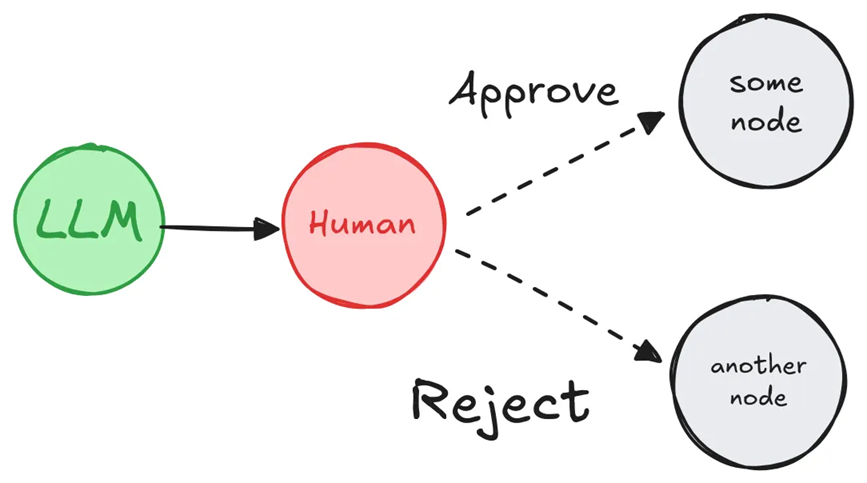
\includegraphics[width=\linewidth,keepaspectratio]{langgraph22}
\end{center}
    \end{column}
  \end{columns}
  
\end{frame}

%%%%%%%%%%%%%%%%%%%%%%%%%%%%%%%%%%%%%%%%%%%%%%%%%%%%%%%%%%%
\begin{frame}[fragile]\frametitle{Human-in-the-Loop: Implementation Patterns}
      \begin{itemize}
        \item \textbf{Pattern 1: Breakpoints}:
        \begin{itemize}
            \item Pause execution at specific nodes
            \item Example: Stop before "send\_email" node
        \end{itemize}
        \item \textbf{Pattern 2: Approval Gates}:
        \begin{itemize}
            \item Node requests approval, waits for response
            \item Conditional edge based on approval status
        \end{itemize}
        \item \textbf{Pattern 3: State Editing}:
        \begin{itemize}
            \item Pause, allow human to modify state
            \item Resume with corrected state
        \end{itemize}
        \item \textbf{Pattern 4: Continuous Monitoring}:
        \begin{itemize}
            \item Human can interrupt at any time
            \item Useful for long-running agents
        \end{itemize}
      \end{itemize}
\end{frame}

%%%%%%%%%%%%%%%%%%%%%%%%%%%%%%%%%%%%%%%%%%%%%%%%%%%%%%%%%%%
\begin{frame}[fragile]\frametitle{Human-in-the-Loop: Code Example}
      \begin{lstlisting}[language=Python, basicstyle=\tiny]
from langgraph.checkpoint.memory import MemorySaver
from langgraph.graph import StateGraph

# Create graph with checkpointing (required for interrupts)
memory = MemorySaver()
workflow = StateGraph(State)

# Add nodes
workflow.add_node("draft_email", draft_email_node)
workflow.add_node("send_email", send_email_node)
# Add edges
workflow.add_edge("draft_email", "send_email")
# Compile with interrupt BEFORE send_email node
app = workflow.compile(
    checkpointer=memory,
    interrupt_before=["send_email"])  # Pause here for human approval
# Run workflow
config = {"configurable": {"thread_id": "1"}}
result = app.invoke(initial_state, config)
# At this point, execution is paused
# Human reviews the drafted email in result.draft
# To resume after approval:
app.invoke(None, config)  # Continues from where it stopped
# To modify state and resume:
updated_state = result.copy()
updated_state.draft = "Modified email content"
app.invoke(updated_state, config)
      \end{lstlisting}
\end{frame}

%%%%%%%%%%%%%%%%%%%%%%%%%%%%%%%%%%%%%%%%%%%%%%%%%%%%%%%%%%%
\begin{frame}[fragile]\frametitle{Advanced Concept: State Persistence and Checkpointing}
      \begin{itemize}
        \item \textbf{What}: Automatically save state at each node execution
        \item \textbf{Benefits}:
        \begin{itemize}
            \item Resume after failures or interruptions
            \item Time-travel debugging (replay from any checkpoint)
            \item Support long-running workflows across sessions
            \item Enable human-in-the-loop patterns
        \end{itemize}
        \item \textbf{Checkpoint Storage Options}:
        \begin{itemize}
            \item In-memory (development/testing)
            \item SQLite (local persistence)
            \item PostgreSQL (production)
            \item Redis (distributed systems)
        \end{itemize}
        \item \textbf{Key Feature}: Each checkpoint is immutable and versioned
        \item Can fork from any checkpoint to explore alternative paths
      \end{itemize}
	  
% \begin{center}
% 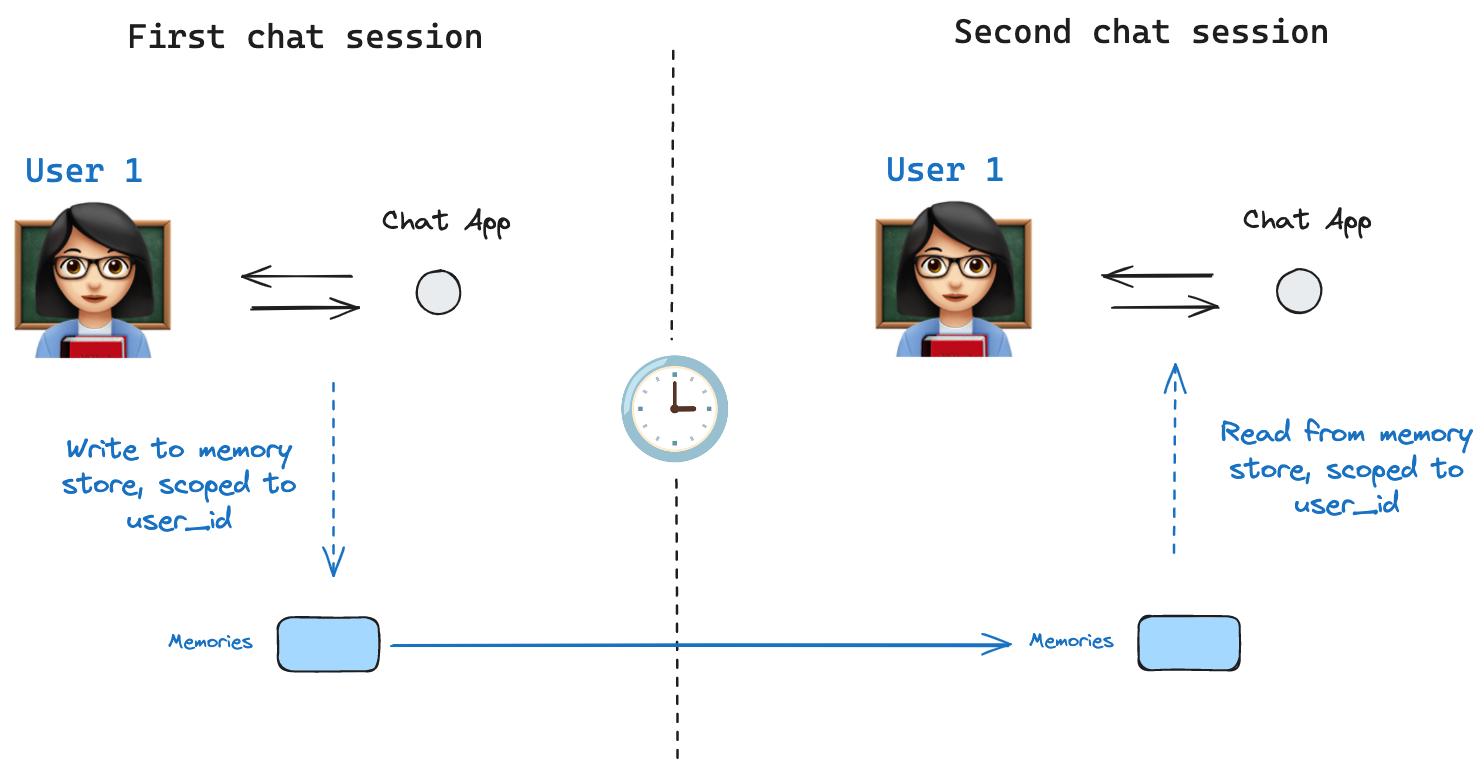
\includegraphics[width=0.6\linewidth,keepaspectratio]{langgraph23}

% {\tiny (Ref: Langgraph docs)}
% \end{center}	  
\end{frame}

%%%%%%%%%%%%%%%%%%%%%%%%%%%%%%%%%%%%%%%%%%%%%%%%%%%%%%%%%%%
\begin{frame}[fragile]\frametitle{Advanced Concept: Streaming and Real-Time Updates}
      \begin{itemize}
        \item \textbf{What}: Stream intermediate results as graph executes
        \item \textbf{Why Important}:
        \begin{itemize}
            \item Provide real-time feedback to users
            \item Show progress in long-running workflows
            \item Better user experience (vs waiting for completion)
        \end{itemize}
        \item \textbf{Streaming Modes}:
        \begin{itemize}
            \item \textbf{values}: Stream complete state after each node
            \item \textbf{updates}: Stream only state changes
            \item \textbf{messages}: Stream LLM token by token
        \end{itemize}
        \item \textbf{Use Case}: Chatbot showing "thinking..." → "searching..." → "responding..."
      \end{itemize}
\end{frame}

%%%%%%%%%%%%%%%%%%%%%%%%%%%%%%%%%%%%%%%%%%%%%%%%%%%%%%%%%%%
\begin{frame}[fragile]\frametitle{Streaming Example}

      \begin{itemize}
        \item Streaming provides transparency into agent execution
        \item Critical for production applications with users waiting
      \end{itemize}
	  
      \begin{lstlisting}[language=Python, basicstyle=\tiny]
# Instead of invoke(), use stream()
for chunk in app.stream(initial_state, config):
    # chunk contains state updates after each node
    print(f"Node: {chunk['node']}")
    print(f"State: {chunk['state']}")
    
# For token-by-token LLM streaming
async for event in app.astream_events(initial_state, config):
    if event["event"] == "on_chat_model_stream":
        # Stream each token as LLM generates
        print(event["data"]["chunk"], end="", flush=True)
      \end{lstlisting}
      

\end{frame}

%%%%%%%%%%%%%%%%%%%%%%%%%%%%%%%%%%%%%%%%%%%%%%%%%%%%%%%%%%%
\begin{frame}[fragile]\frametitle{Advanced Concept: Subgraphs and Modularity}
      \begin{itemize}
        \item \textbf{What}: Embed complete graphs as nodes within parent graphs
        \item \textbf{Benefits}:
        \begin{itemize}
            \item Modular, reusable workflow components
            \item Hierarchical organization of complex systems
            \item Encapsulation and separation of concerns
        \end{itemize}
        \item \textbf{Example Hierarchy}:
        \begin{itemize}
            \item Parent: Customer service orchestrator
            \item Subgraph 1: Email classification workflow
            \item Subgraph 2: Ticket routing workflow
            \item Subgraph 3: Response generation workflow
        \end{itemize}
        \item Each subgraph is self-contained with own state and logic
        \item Parent graph coordinates between subgraphs
        \item Enables building complex systems from simple components
      \end{itemize}
\end{frame}

%%%%%%%%%%%%%%%%%%%%%%%%%%%%%%%%%%%%%%%%%%%%%%%%%%%%%%%%%%%
\begin{frame}[fragile]\frametitle{Advanced Concept: Parallel Execution}
      \begin{itemize}
        \item \textbf{What}: Execute multiple nodes simultaneously
        \item \textbf{Use Cases}:
        \begin{itemize}
            \item Call multiple APIs concurrently
            \item Search multiple data sources in parallel
            \item Generate multiple variations simultaneously
        \end{itemize}
        \item \textbf{Implementation}: Send edges from one node to multiple nodes
      \end{itemize}
      
      \begin{lstlisting}[language=Python, basicstyle=\small]
# Parallel node execution
workflow.add_node("search_web", search_node)
workflow.add_node("search_db", database_node)
workflow.add_node("search_docs", documents_node)
workflow.add_node("aggregate", aggregate_results)
# Fan-out: one node to many
workflow.add_edge("start", "search_web")
workflow.add_edge("start", "search_db")
workflow.add_edge("start", "search_docs")
# Fan-in: many nodes to one
workflow.add_edge("search_web", "aggregate")
workflow.add_edge("search_db", "aggregate")
workflow.add_edge("search_docs", "aggregate")
      \end{lstlisting}
\end{frame}

%%%%%%%%%%%%%%%%%%%%%%%%%%%%%%%%%%%%%%%%%%%%%%%%%%%%%%%%%%%
\begin{frame}[fragile]\frametitle{Advanced Concept: Dynamic Graph Modification}
      \begin{itemize}
        \item \textbf{What}: Modify graph structure during execution
        \item \textbf{Use Cases}:
        \begin{itemize}
            \item Add nodes based on runtime conditions
            \item Dynamically adjust workflow based on results
            \item Create adaptive systems that evolve
        \end{itemize}
        \item \textbf{Example Scenario}:
        \begin{itemize}
            \item Research agent discovers new sub-topics
            \item Dynamically creates specialized research nodes
            \item Each node investigates a different aspect
        \end{itemize}
        \item \textbf{Limitation}: Advanced feature, use with caution
        \item Most use cases handled by conditional edges
        \item True dynamic modification for special scenarios only
      \end{itemize}
\end{frame}

%%%%%%%%%%%%%%%%%%%%%%%%%%%%%%%%%%%%%%%%%%%%%%%%%%%%%%%%%%%
\begin{frame}[fragile]\frametitle{Advanced Patterns: Map-Reduce}
      \begin{itemize}
        \item \textbf{Pattern}: Split work, process in parallel, combine results
        \item \textbf{Example - Document Summarization}:
        \begin{enumerate}
            \item Split large document into chunks (map)
            \item Summarize each chunk in parallel (parallel processing)
            \item Combine summaries into final summary (reduce)
        \end{enumerate}
        \item \textbf{Implementation}:
        \begin{itemize}
            \item Split node: Divides input into subtasks
            \item Multiple processing nodes: Execute in parallel
            \item Aggregation node: Combines results
        \end{itemize}
        \item \textbf{Benefits}: Scalability, speed, handles large inputs
        \item Common in RAG systems for processing multiple documents
      \end{itemize}
\end{frame}

%%%%%%%%%%%%%%%%%%%%%%%%%%%%%%%%%%%%%%%%%%%%%%%%%%%%%%%%%%%
\begin{frame}[fragile]\frametitle{Best Practices for Advanced Features}
      \begin{itemize}
        \item \textbf{Start Simple}: Add complexity only when needed
        \item \textbf{Checkpointing}: Always use for production systems
        \item \textbf{Error Handling}: Add try-except in nodes, fallback paths in graph
        \item \textbf{Observability}: Use LangSmith/Langfuse to trace execution
        \item \textbf{Testing}: Test nodes individually, then integration test graphs
        \item \textbf{State Size}: Keep state minimal - only essential data
        \item \textbf{Cycle Limits}: Set maximum iterations to prevent infinite loops
        \item \textbf{Human Approval}: For high-stakes actions (financial, emails, deletions)
        \item \textbf{Documentation}: Graph visualization helps team understanding
      \end{itemize}
\end{frame}

%%%%%%%%%%%%%%%%%%%%%%%%%%%%%%%%%%%%%%%%%%%%%%%%%%%%%%%%%%%%%%%%%%%%%%%%%%%%%%%%%%
\begin{frame}[fragile]\frametitle{Summary}
      \begin{itemize}
        \item LangGraph enables controlled, flexible AI workflows through graph structures
        \item Solves limitations of rigid chains and unpredictable pure agents
        \item Key components: Nodes (logic), Edges (flow), State (context)
        \item Ideal for workflow automation with intelligent decision-making
        \item Production-ready with state persistence, human-in-loop, streaming
        \item Start with simple workflows, expand to complex multi-agent systems
        \item The future of reliable, autonomous AI applications
      \end{itemize}
\end{frame}